\documentclass[12pt]{report}
\usepackage{commands}
\newenvironment{problem}{}{\newpage}


\begin{document}

\large
\begin{center}
AMSC 660 Final Exam\\
Due 12/18/23\\
By Marvyn Bailly\\
\end{center}
\normalsize
\hrule

%Good luck my man
%---------------%
%---Problem 1---%
%---------------%


\begin{problem}%[vskip]
\subsection*{Problem 1}

Think about a maze similar to the one in Problem 5 of HW7. It is helpful to read the entire statement of Problem 5 in HW7 for solving this problem.
The maze consists of an $n \times n$ array of cells. The connectivity of the maze is described by an adjacency matrix $A$ of size $N \times N$ where $N = n^2$. $A_{ij} = 1$ if cells $i$ and $j$ are adjacent and there is no wall between them, and $A_{ij} = 0$ otherwise. We assume that the maze is connected, i.e., there is a path between any pair of cells. In particular, there is a path from the top left cell indexed by 1 and the bottom right cell indexed by $N$. Note that the matrix $A$ is symmetric.

As in problem 5 of HW7, we compute row sums of $A$ and convert the adjacency matrix $A$ into a stochastic matrix $P$:

\begin{equation}
P = R^{-1}A, \quad \text{where} \quad R = \text{diag} \left( \sum_{j=1}^{N} A_{1j}, \ldots, \sum_{j=1}^{N} A_{Nj} \right).
\end{equation}

\begin{enumerate}
    \item \textbf{(4 pts)} Prove that all eigenvalues of $P$ are real.\\
  \textit{Hint: Start with the identity $PV = V \Lambda$ where $V$ is the matrix whose columns are the eigenvectors of $P$ and $\Lambda$ is the diagonal matrix with the corresponding eigenvalues of $P$ along its diagonal.}
    
    \item \textbf{(2 pts)} The eigenvectors of $P$ are, generally, not orthogonal with respect to the dot product, i.e., $V^T V \neq I$, where $I$ is the $N \times N$ identity matrix. Find a symmetric positive definite matrix $?$ such that $V^T(?)V = I_{N \times N}$ where $V$ is the matrix whose columns are the eigenvectors of $P$, i.e., the eigenvectors of $P$ are orthogonal with respect to the $?$-inner product.
    
    \item \textbf{(4 pts)} Evidently, the matrix $L := P - I$ is not invertible because its row sums are all equal to zero. However, in problem 5, HW7, we solved a linear system whose matrix $\tilde{L}$ was obtained from $L$ by removing the first and the last row and the first and the last column of $L$:
    \begin{equation}
        \tilde{L} := L_{2:(N-1),2:(N-1)}.
    \end{equation}
    
    Prove that the matrix $\tilde{L}$ is invertible.
    
    \textit{Hint: Proceed from converse. Assume that there is $x \in \mathbb{R}^{N-2}, x \neq 0$, such that $\tilde{L}x = 0$, i.e., $x$ is the eigenvector corresponding to the zero eigenvalue of $\tilde{L}$. Normalize $x$ so that its maximal entry in absolute value equals 1. Now observe that $\tilde{L}x = 0$ is equivalent to $x = \tilde{P}x$. Recall that $P$ is irreducible, i.e., each pair of sites is connected by a path in the maze (the maze can be thought of as a graph). This means that there is a sequence connecting any pair of sites $i$ and $j$,}
    \[
    (i, k_1), (k_1, k_2), \ldots, (k_s, j)
    \]
    \textit{such that the entries of $P$ with subscripts in this sequence are positive.}
    
    
\end{enumerate}

\subsection*{Solution}
\begin{proof}
Consider the $N \times N$ matrix $A$ where $A$ is symmetric and its entries are either $0$ or $1$. We define the stochastic matrix $P$ as follows: 
\begin{equation*}
    P = R^{-1}A, \quad \text{where} \quad R = \text{diag} \left( \sum_{j=1}^{N} A_{1j}, \ldots, \sum_{j=1}^{N} A_{Nj} \right).
\end{equation*}
\begin{enumerate}
    \item 
    We wish to show that the eigenvalues of $P$ are real. Note that since $A$ is real and symmetric, $A = \overline{A}$, making $A$ hermitian. Since all hermitian matrices have real and positive eigenvalues \footnote{The proof follows easily using inner products: let $(\lambda,v)$ and an eigenpair for $A$ hermitian, then $\lambda \abrac{v,v} = \abrac{\lambda v, v} = \abrac{Av,v} = \abrac{v,A^{\dagger}v} = \abrac{v,Av} = \abrac{v,\lambda v} = \overline{\lambda}\abrac{v,v}$, so $\lambda = \overline{\lambda}$ as $v\neq 0$ gives $\abrac{v,v} \neq 0$.}, so does $A$. We also note that since $R$ is diagonal, so is $R^{-1}$ and thus $R^{-1}$ is symmetric. Let $(\lambda,v)$ be an eigenpair for $P$ which gives the following equivalences:
    \begin{equation*}
        Pv = \lambda v \iff R^{-1}Av = \lambda v \iff Av = \lambda Rv.
    \end{equation*}
    Now we can take the complex conjugate to get
    \begin{equation*}
        \overline{Av} = \overline{\lambda Rv} \iff A\overline{v} = \overline{\lambda}R\overline{v}.
    \end{equation*}
    Observe that 
    \begin{align*}
          (\lambda Rv)^\top &= (Av)^\top\\ 
        \lambda v^\top R &= v^\top A \\
        \lambda v^\top R \overline{v} &= v^\top A \overline{v}\\
        \lambda v^\top R \overline{v} &= v^\top \paren{\overline{\lambda}R\overline{v}}\\
        \overline{\lambda} \paren{v^\top R\overline{v}} &= \lambda \paren{v^\top R \overline{v}}.
    \end{align*}
    Notice that by the construction of $R$, for $\mathbf{x}=\brac{x_1,\dots,x_N}^\top$, we get
    \begin{equation*}
        \mathbf{x}^\top R \overline{\mathbf{x}} = \sum_{i=1}^N \sum_{j=1}^N A_{i j} x_i\overline{x_i} = \sum_{i=1}^N \sum_{j=1}^N A_{i j} |x_i|^2 \geq 0,
    \end{equation*}
    where we have greater than equal to zero since $A_{i j} \in \brac{0,1}$ and we achieve equality if and only if $\mathbf{x} = \mathbf{0}$. Therefore $\paren{v^\top R\overline{v}} > 0$ since $v \neq 0$ and so $\overline{\lambda} = \lambda$ which is only true if $\lambda \in \R$. Since this holds for an arbitrary eigenpair of $P$, we have shown that all eigenvalues of $P$ are real. 


    \item
    Let $PV = V \Lambda$ be the eigendecomposition where $V$ is the matrix whose columns are the eigenvectors of $P$ and $\Lambda$ is the diagonal matrix with the corresponding eigenvalues of $P$ along its diagonal. We wish to find a symmetric positive definite matrix $B$ such that $V^\top B V = I_{N \times N}$, the $N \times N$ identity matrix. In other words, we are searching for a matrix $B$ such that
    \begin{equation*}
        (V^T B V)_{ij} = v_j^\top B v_i = \begin{cases}
            1 &\text{if } i = j,\\
            0 &\text{otherwise.}
        \end{cases}
    \end{equation*}
    If $V$ is  full rank, then $V$ is invertible and there are a couple options for $B$. We could let $B =W^\top W$ where $W = V^{-1}$. Then $B$ is symmetric since $B^\top = (W^\top W)^\top = W^\top W$ and is symmetric since $V$ is full rank, then so is $W$, meaning that $Wx = 0$ only if $x=0$. Furthermore, 
    \begin{equation*}
        x^\top B x = x^\top W^\top W x = (Wx)^\top (Wx) \geq 0,
    \end{equation*}
    by definition of the dot product where equality is achieved only if $x = 0$. Therefore $B$ is SPD and we also have
    \begin{equation*}
        V^\top B V = V^\top V^{-\top} V^{-1} V = I,
    \end{equation*}
    as desired. 

    \noindent
    Another choice could be to let $B = \text{diag}(\|v_1\|^{-2},\dots,\|v_N\|^{-2})$. Since this matrix is diagonal, it is symmetric and since the elements along the main diagonal are positive, $B$ is positive definite, thus $B$ is SPD (proof omitted since it follows the proof that $R$ is SPD). Then we have that for $i\neq j$, since the eigenvectors are orthogonal, $v_i^\top B v_j = 0$ and for $i = j$ we have $\|v_i\|^2 b_ii = 1$ making $V^\top B V = I$.
    
    \noindent
    On the other hand, if $V$ is not full rank, neither of the above methods will work. So let's try using $R$ which is SPD as it has nonnegative values along the main diagonal. To see why this makes $R$ SPD, observe that 
    for $\mathbf{x}=\brac{x_1,\dots,x_N}^\top$, we get
    \begin{equation*}
        \mathbf{x}^\top R \mathbf{x} = \sum_{i=1}^N \sum_{j=1}^N A_{i j} x_i^2 \geq 0,
    \end{equation*}
    where equality is achieved if and only if $\mathbf{x} = \mathbf{0}$. Then we have that
    \begin{equation*}
        (V^T R V)_{ij} = v_j^\top R v_i.
    \end{equation*}
    To see that this yields the desired identity matrix, observe that for an arbitrary $j$ and $i$ we can write
    \begin{equation*}
        Pv_i = \lambda_i v_i \iff Av_i = \lambda_i R v_i \iff v_j^\top Av_i = \lambda_i v_j^\top R v_i,
    \end{equation*}
    and
    \begin{equation*}
        Pv_j = \lambda_j v_j \iff A_j v_j = \lambda_j R v_j \iff v_j^\top A_j = \lambda_j v_j^\top R \iff v_j^\top A_j v_i = \lambda_j v_j^\top R v_i. 
    \end{equation*}
    Combining these two expressions, yields 
    \begin{equation*}
        0 = \paren{\lambda_i - \lambda_j}v_j^\top R v_i,
    \end{equation*}
    so if $i \neq j$, then $v_j^\top R v_i = 0$ and if $i = j$, then $v_j^\top R v_i$ could be nonzero. Then if we normalize $R$, we will have ones along the diagonal assuming that $v_j^\top R v_i \neq 0$. I also realize that this requires the eigenvalues of $P$ to be distinct, which implies that $V$ is full rank so this method only works if $V$ is full rank.

    \textit{Note:} I ran out of ideas on how to show this holds if $V$ is rank deficient.

    \item
    Consider the matrix $L := P - I$ which is not invertible but by removing the first and last row and the first and last column of $L$:
    \begin{equation*}
        \tilde{L} := L_{2:(N-1),2:(N-1)} = P_{2:(N-1),2:(N-1)} - I_{N-2\times N-2} = \tilde{P} - \tilde{I},
    \end{equation*}
    $\tilde{L}$ is invertible. We wish to formally prove this. Let's assume the converse, then there exists $x \in \R^{N -2}$ such that $x \neq 0$  and $\tilde{L}x = 0$. Without loss of generality, let's normalize $x$ such that the maximal entry in absolute value is equal to $1$ (A similar argument could be made if the maximal entry is $-1$). Now recall that $P$ by construction has a path from the top cell, $P_{1,1}$, to the bottom right cell, $P_{N,N}$. Since $P$ is irreducible, this means that $P_{1,2},P_{2,1},P_{N,N+1},P_{N+1,N} \neq 0$ and since $P$ is stochastic, this means that the row sum of the second and second to last row of $P$ are strictly less than zero. Now returning to $\tilde{P}$, we have that the row sum of the first and last row are strictly less than $1$. We also have that $|x_i| \leq 1$ for all $i$. But then there is no way for 
    \begin{equation*}
        \tilde{P}x = x \iff x_j = \sum_{i=1}^{N_2}P_{j,i}x_j,
    \end{equation*}
    if $\tilde{P}$ has row sums less than while and $|x_i| \leq 1$. Thus we have found a contradiction showing that if $\tilde{L}x = 0,$ then $x=0$. This implies that $\tilde{L}$ is invertible as desired.\footnote{The proof is not as rigorous as I had hoped, but I ran out of time.}
    
    \textit{Potential Proof that but doesn't use hint:} To show that $\tilde{L}$ is invertible, we assume that it isn't,

    \textit{Note:} I came up with this argument but this would also show that $L$ is irreducible which is confusing to me but I can't find where this proof is incorrect: Now since $\tilde{L}=\tilde{P}-\tilde{I}$, we get 
    \begin{equation*}
        \tilde{L}x = \tilde{P}x - x = 0,
    \end{equation*}
    so $\tilde{P}x = x$. Recall that $P = R^{-1}A$ so consider $\tilde{P} = \tilde{R^{-1}}\tilde{A}$, where the tilde denotes the removing of the first and last column and first and last row. This gives that
    \begin{equation*}
        \tilde{P}x = x \iff \tilde{R^{-1}A}x = x \iff \tilde{A}x = \tilde{R}x \iff \tilde{A}xx^{-1} = \tilde{R}xx^{-1} \iff \tilde{A} = \tilde{R},
    \end{equation*}
    which means that $\tilde{A}$ must be diagonal as $\tilde{R}$ is diagonal. But this implies that $\tilde{P} = \tilde{R}^{-1}\tilde{A}$ is diagonal which contradicts $\tilde{P}$ being irreducible since there is no path between the diagonal elements. Therefore, if $\tilde{L}x = 0$, then $x = 0$ which shows that $\tilde{L}$ is invertible. 

\end{enumerate}

\end{proof}
\end{problem}




%---------------%
%---Problem 2---%
%---------------%


\begin{problem}%[vskip]
\subsection*{Problem 2}

Depicting graphs nicely is important as some properties of a graph can be first detected by visual inspection.

\textbf{(10 pts)} We consider an approach based on minimizing an energy function for a graph. An unweighted undirected graph \(G(V, E)\) consists of a set of vertices \(V = \{1, \ldots, N\}\) a set of edges \(E \subset \{(i,j) | i,j \in V\}\). A graph \(G(V, E)\) can be defined by its adjacency matrix \(A\):
\begin{equation}
    A_{i,j} = 
    \begin{cases} 
1, & (i,j) \in E \\
0, & \text{otherwise}
\end{cases}
\quad 1 \leq i,j \leq N.
\end{equation}
Since the graph is undirected, \(A\) is symmetric.

In a depiction of a graph, we want all linked vertices to be at a distance of 1 from each other, while all unlinked vertices at a distance of at least as large as \(\sqrt{3}\) of each other. The value \(\sqrt{3}\) is motivated by the distance between unlinked vertices in a right hexagon with side 1. Motivated by this wish, we set up the following energy function

\begin{align}
    U(x,y) &= \frac{1}{2} \sum_{(i,j) \in E} \left( \sqrt{(x_i - x_j)^2 + (y_i - y_j)^2} - 1 \right)^2\\
    &+ \frac{1}{2} \sum_{(i,j) \notin E} \left( \sqrt{(x_i - x_j)^2 + (y_i - y_j)^2} - \sqrt{3} \right)^2_{-}, \nonumber
\end{align}
where $x, y \in \mathbb{R}^N$, and
\begin{equation}
    \left( \sqrt{(x_i - x_j)^2 + (y_i - y_j)^2} - \sqrt{3} \right)_{-} = \min \left\{ \sqrt{(x_i - x_j)^2 + (y_i - y_j)^2} - \sqrt{3}, 0 \right\} 
\end{equation}
The first sum is the sum of spring energies for all edges of the graph while the second sum is the sum of all repelling spring energies of unlinked vertices. The corresponding force,
\begin{equation*}
    f (x, y) = -\nabla U (x, y),
\end{equation*}
is implemented in Matlab and Python functions called forces. To avoid large force when the linked vertices are far from each other, these routines cap the absolute value of each component of the attracting forces due to links by 1. 

\textbf{Task.} Write a code that computes the positions of vertices of a graph and draws it. You need to choose any appropriate deterministic optimizer except for the gradient descent out of those that we have studied (BFGS line search, BFGS trust region, Nesterov, Adam, Levenberg-Marquardt). The graph to test your code is defined by an adjacency matrix in the file \verb+Adjacency_matrix.csv+.  The graph has $N = 91$ vertices. The initial positions of the vertices can be chosen e.g. as Gaussian random variables with mean zero and standard deviation $N$. You should obtain something like the graph in Fig. 1. My graph plotting routines are provided in Matlab and Python functions \verb+plot_graph+. Please feel free to write your own plotting routine. In this case, make sure to set an equal aspect ratio and turn the axes off. Also, you are welcome to modify the energy function in any reasonable manner as soon as the resulting graph depiction satisfies the guideline highlighted in italics above.

\textit{Submit the resulting figure of the graph, specify which optimizer you implemented, and include the progress report for the optimizer. Plot the norm of the force versus iteration number in log scale along the $y$-axis and print the norm of the residual every once in a while. Link your code to your pdf file.}



\subsection*{Solution}
\begin{proof}
Consider the energy function 
\begin{align*}
    U(x,y) &= \frac{1}{2} \sum_{(i,j) \in E} \left( \sqrt{(x_i - x_j)^2 + (y_i - y_j)^2} - 1 \right)^2\\
    &+ \frac{1}{2} \sum_{(i,j) \notin E} \left( \sqrt{(x_i - x_j)^2 + (y_i - y_j)^2} - \sqrt{3} \right)^2_{-}, \nonumber
\end{align*}
where $x, y \in \mathbb{R}^N$, and
\begin{equation*}
    \left( \sqrt{(x_i - x_j)^2 + (y_i - y_j)^2} - \sqrt{3} \right)_{-} = \min \left\{ \sqrt{(x_i - x_j)^2 + (y_i - y_j)^2} - \sqrt{3}, 0 \right\}.
\end{equation*}
We are given the \verb+force.m+ file which computes
\begin{equation*}
    f(x,y) = - \nabla U(x,y).
\end{equation*}
Since we are already given a function to find the gradient, let's implement an optimizer that utilizes the gradient without needing the function values. Out of our options, these would be the deterministic form of Nesterov and Adam. Let's use Adam's method which we implement in Matlab using the following code: 
\begin{lstlisting}[style=Matlab-editor]
function [w,gnorm] = adams(grad, w, kmax, tol,N)
    gnorm = zeros(kmax, 1); 
    beta1 = 0.9;
    beta2 = 0.999; 
    e = 10e-8;
    alpha = 0.001;
    m = zeros(length(w),1);
    v = zeros(length(w),1);
    
    for k = 1:kmax
        g = -grad(w(1:N),w(N+1:end));
        gnorm(k) = norm(g);

        m = beta1 * m + (1 - beta1).*g;
        v = beta2 * v + (1 - beta2).*g.^2;

        mt = m ./ (1 - beta1^k);
        vt = v ./ (1 - beta2^k);
        
        w = w -  alpha*mt ./ (sqrt(vt)  + e);
        
        % Print progress every 5000 iteration
        if mod(k,5000)==0
            fprintf('k = %d, gnorm = %d\n',k,gnorm(k))
        end
        % Check for convergence
        if gnorm(k) < tol
            break;
        end
    end
    gnorm = gnorm(1:k);
    fprintf('Ended at k = %d with gnorm = %d\n',k,gnorm(k))
end  
\end{lstlisting}
which returns the minima of the energy function, prints the norm of the gradient every $5000$th iteration, and a list corresponding to the  gradient norm on each iteration. We generate the initial positions of the vertices with a Gaussian random vector with mean zero and standard deviation $N$. Note, that since \verb+forces.m+ file takes $(x,y)$, we concatenate the vector as $\mathbf{w} = (x,y)^\top$ and run the Adam's optimizer on $\mathbf{w}$. Running the code with a tolerance of $10^{-4}$ and a max iteration count of $10^{5}$ terminates on the $22150$ iteration with a residual of $9.922146e-05$ and yields Table \ref{tablefor1} and Figure \ref{fig1}. From Table \ref{tablefor1} and Figure \ref{fig1}, we see that the optimizer rapidly converges to the minima with minimal bouncing around. Note, we picked a tolerance of $10^{-4}$ since the Adams method was unable to find a smaller residual which we can see by the noisy $\nabla U$ values around $2\times 10^4$ iterations before the algorithm converges. We can visualize the result of the graph as seen in Figure \ref{fig2}, which looks very nice. 

\noindent
Complete code can be found at \url{https://github.com/MarvynBailly/AMSC660/blob/main/final/question2.m} 

\begin{table}[h!] 
    \center
    \begin{tabular}{c|lllll}
     Iteration &  $5000$&  $10000$& $15000$ & $20000$ & $22150$\\ \hline
     $\nabla U $& $4.724460$ & $1.851327$ & $.6491553$ &  $4.223797\times 10^{-03}$ & $9.922146\times10{-05}$\\ 
    \end{tabular}
    \caption{The $\nabla U$ value on every $5000$th iteration of the Adams method and the final iteration it converged on.}
    \label{tablefor1}
\end{table}

\begin{figure}[h!]
    \centering
    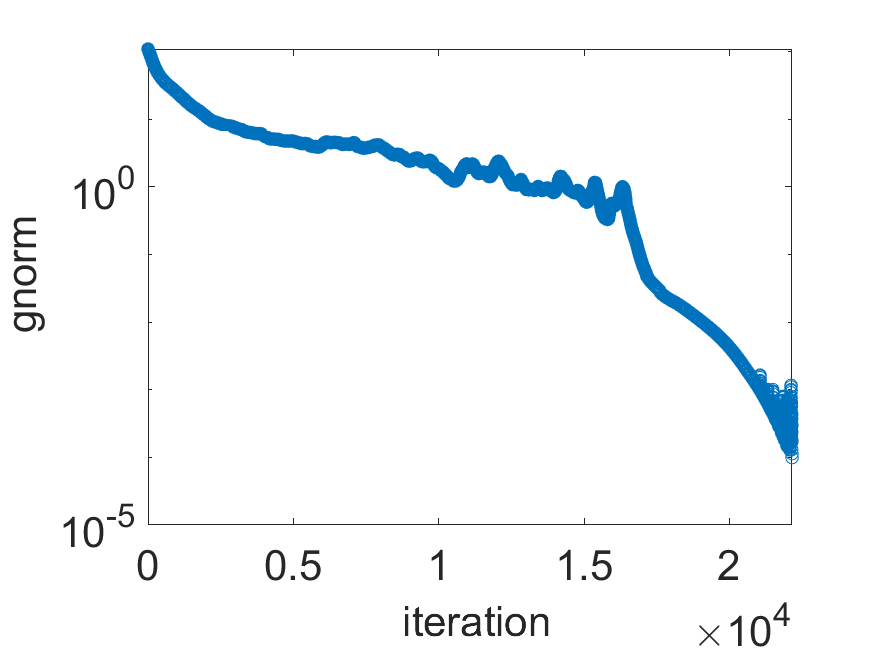
\includegraphics[width=0.75\textwidth,height=\textwidth,keepaspectratio]{images/coolplot2.png}
    \caption{Plot showing $\nabla U$ value on each iteration using the Adams method.}
    \label{fig1}
\end{figure}

\begin{figure}[h!]
    \centering
    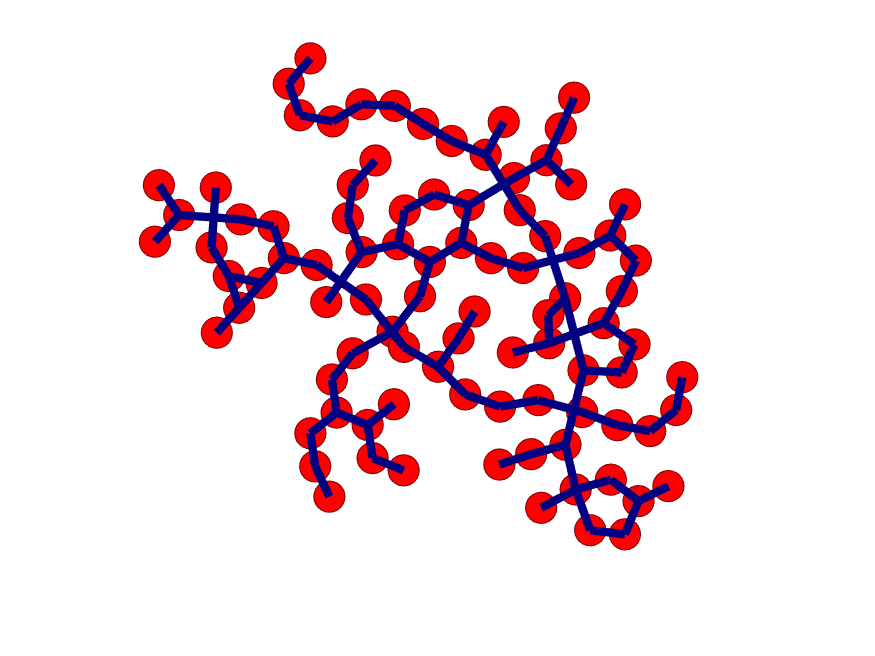
\includegraphics[width=0.75\textwidth,height=\textwidth,keepaspectratio]{images/coolplot1.png}
    \caption{A depiction of the graph found using Adams method.}
    \label{fig2}
\end{figure}


\end{proof}
\end{problem}


%---------------%
%---Problem 3---%
%---------------%


\begin{problem}%[vskip]
\subsection*{Problem 3}

\textbf{(10 pts)}
\begin{enumerate}
    \item Consider a 2D Ising model on a square lattice with periodic boundary conditions. Find the change in energy, \(\Delta H = H_{\text{new}} - H\), resulting from flipping a spin at site \((i,j)\). Your expression should involve only the spin at \((i,j)\) and its nearest neighbors.
    \item Write a code to compute the mean magnetization \(\mu(\beta)\) for the 2D Ising model by the Metropolis algorithm. Use a \(30 \times 30\) lattice with the periodic boundary conditions, i.e., the nearest neighbors of site \((i,j)\) where \(0 \leq i,j \leq 29\) are \((i \pm 1 \mod 30, j \pm 1 \mod 30)\). Your program should compute the running mean and the running variance of the magnetization. These quantities are defined, respectively, by
    \[
    \overline{m}_k = \frac{1}{k} \sum_{i=1}^{k} m_i, \quad [\text{Var}(m)]_k = \frac{1}{k - 1} \sum_{i=1}^{k} (m_i - \overline{m}_i)^2,
    \]
    where \(k\) is the current number of iterations. Note that you do not need to store all values of the magnetization. You need only to update \(\overline{m}_k\) and \(\text{Var}(\overline{m}_k)\) using the new value of \(m\) and the running mean \(\overline{m}_k\) at each iteration.
    \item Recall that the analytic expression for the mean magnetization is
    \begin{equation}
        \mu(\beta) = 
        \begin{cases}
        \left(1 - \sinh(2\beta)^{-4}\right)^{1/8}, & \beta > 1/T_c = 0.4408, \\
        0, & \beta < 1/T_c = 0.4408.
        \end{cases}     
    \end{equation}
    Use your code to calculate \(\mu\) for the set of values of \(\beta = 0.2:0.1:1\). Initially, set all spins up for each value of \(\beta\). Desirably, use \(k_{\text{max}} = 10^8\) iterations for each value of \(\beta\). You can use a smaller number of iterations while debugging and then run your code overnight with \(k_{\text{max}} = 10^8\). If your computer is slow, please feel free to reduce \(k_{\text{max}}\) appropriately.

    Plot the graph of the computed mean magnetization as a function of \(\beta\) and superimpose it with the graph of \(\mu(\beta)\) given by Eq. (6). Also plot \(\overline{m} \pm \sqrt{\text{Var}(\overline{m})}\).

    Submit your derivation for Question 1, your plot, and link your code to your pdf file.
\end{enumerate}


\subsection*{Solution}
\begin{proof}
    Consider the 2D Ising model on an $N\times N$ grid with periodic boundary conditions.
\begin{enumerate}
    \item  We wish to find the change in energy $\Delta H = H_{\text{new}} - H$ resulting from flipping a spin at site $(i,j)$. Recall that the spin at each site $(i,j)$ can either be up $s_{i,j} = 1$ or down $s_{i,j} = -1$ and that the total energy system is the sum of energies of the magnetic interactions of the spins $s_{i,j}$ at the nearest neighbors of the grid is given by
    \begin{equation*}
        H\paren{\brac{S_{ij}}} = -\sum_{i,j = 0}^{N -1}s_{ij}(s_{i +1,j} + s_{i,j+1}),
    \end{equation*}
    where the addition in the indices is module $N$ to account for the boundary conditions. To find the change in energy, let the spin at $(i,j)$ be $s_{i,j}$, so flipping $(i,j)$ will result in $-s_{i,j}$. Thus we get that
    \begin{align*}
        \Delta H &= H_\text{new} - H\\
                &= -\paren{\sum_{m,n \neq i,j}^{N -1}s_{mn}(s_{m +1,n} + s_{m,n+1}) + \paren{-s_{ij}(s_{i+1,j} + s_{i,j+1} + s_{i-1,j} + s_{i,j-1})}}\\
                &+ \paren{\sum_{m,n \neq i,j}^{N -1}s_{mn}(s_{m +1,n} + s_{m,n+1}) + s_{ij}(s_{i+1,j} + s_{i,j+1} + s_{i-1,j} + s_{i,j-1})}\\
                &= s_{ij}(s_{i+1,j} + s_{i,j+1} + s_{i-1,j} + s_{i,j-1}) + s_{ij}(s_{i+1,j} + s_{i,j+1} + s_{i-1,j} + s_{i,j-1})\\
                &=2s_{ij}(s_{i+1,j} + s_{i,j+1} + s_{i-1,j} + s_{i,j-1}).
    \end{align*}
    Therefore,  $\Delta H = 2s_{ij}(s_{i+1,j} + s_{i,j+1} + s_{i-1,j} + s_{i,j-1})$ when flipping the spin at site $(i.j)$.


    \item We will use the Metropolis algorithm to compute the running mean and running variance of the magnetization. We implement the Metropolis algorithm in Matlab as follows:
    \begin{lstlisting}[style=Matlab-editor]
function [mu,var] = Metropolis(mesh,beta,iterMax)
    N = length(mesh);
    % compute magnetization
    m = sum(mesh,'all')/N^2;
    mu = m;
    var = 0;

    for iter = 1:iterMax
        % randomly pick a site, flip, and compute difference
        k = randi(N);
        l = randi(N);
        
        % compute delta H
        Dh = 2*mesh(k,l)*(mesh(mod(k-2, N) + 1, l) + mesh(mod(k, N) + 1, l) + mesh(k, mod(l-2, N) + 1) + mesh(k, mod(l, N) + 1));
        
        % if we accept this one, update the spins
        % note the rand is U(0,1)
        if Dh < 0 || rand < exp(-beta*Dh)
            mesh(k,l) = -mesh(k,l);
            % update the magnetization
            m = sum(mesh,'all')/N^2;
        end
    
        % update the running mean
        mu = (iter*mu+m)/(iter+1);
            
        % update the running variance
        var = ((iter - 1) * var + (m - mu)^2) / iter;
    end
end
    \end{lstlisting}
    Here we use the running mean and variance to avoid storing all the values of the magnetization.


    \item
    Now we consider a $30\times 30$ lattice and run the method for $\beta = 0.1 : 0.01 : 1$. Initially, we set all the spins up for and use a max iteration count of $k_\text{max} = 10^8$ each $\beta$ value. Plotting the graph of the computed mean magnetization as a function of \(\beta\) and superimposing it with \(\overline{m} \pm \sqrt{\text{Var}(\overline{m})}\) and the graph of \(\mu(\beta)\) given by 
    \begin{equation*}
        \mu(\beta) = 
        \begin{cases}
        \left(1 - \sinh(2\beta)^{-4}\right)^{1/8}, & \beta > 0.4408, \\
        0, & \beta < 0.4408,
        \end{cases}     
    \end{equation*}
    yields Figure \ref{fig3} and we see that the method is able to match the analytical expression pretty well and recovers the bifurcation at $\beta = 1/T_c = 0.4408$. Complete code can be found at \url{https://github.com/MarvynBailly/AMSC660/blob/main/final/question3.m}


    \begin{figure}[H]
        \centering
        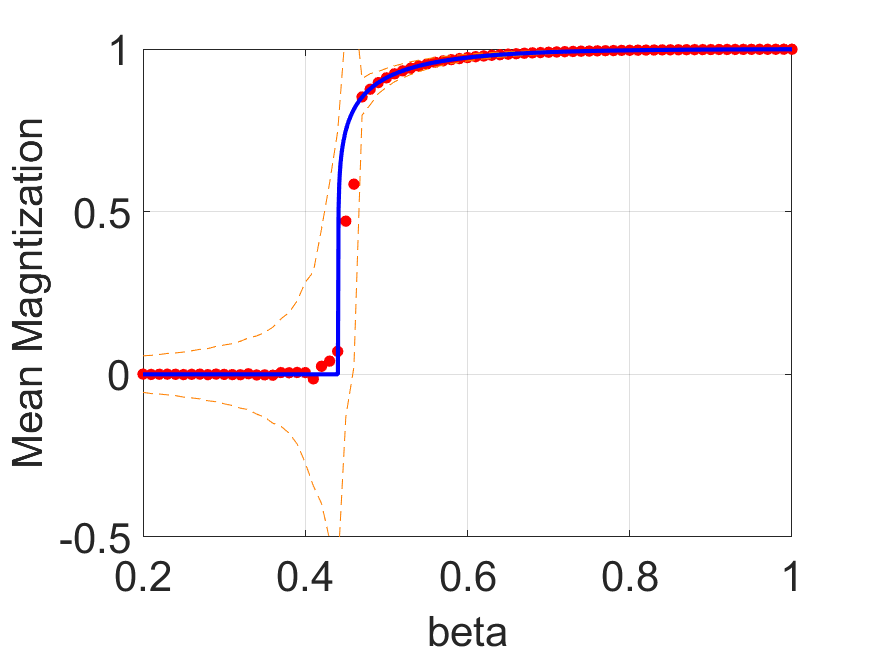
\includegraphics[width=0.75\textwidth,height=\textwidth,keepaspectratio]{images/coolplot3.png}
        \caption{In blue we see the analytical solution $\mu(\beta)$, the red dots are the mean magnetization found by the algorithm, and the dotted orange shows the computed magnetization $\pm$ standard deviation.}
        \label{fig3}
    \end{figure}

    
\end{enumerate}

\end{proof}
\end{problem}






\end{document}